\section{Rhino Command Usage}

\begin{enumerate}
    \item To start the Rhino plugin, run the command \textit{ApplyRulePackage}.\\
    \begin{minipage}{\linewidth}
        \centering
        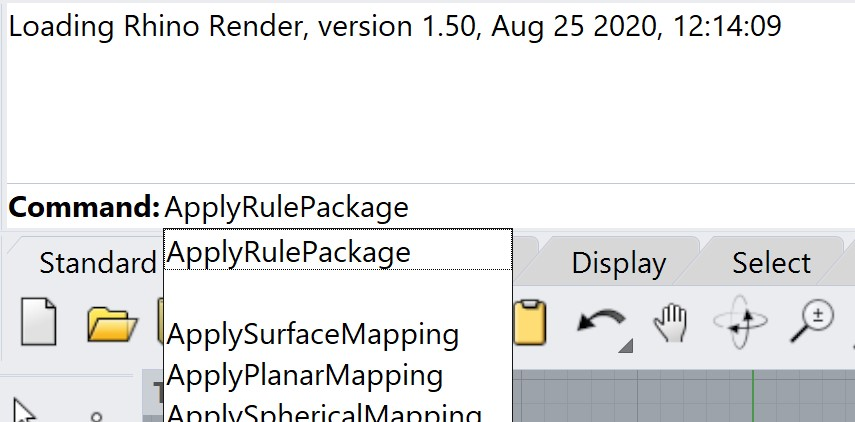
\includegraphics[width=10cm]{res/man_rhino_cmd}
        \captionof{figure}{The Rhino Command.}
    \end{minipage}
    \item It will open the file browser. Select a rule package (.rpk) and click open.\\
    \begin{minipage}{\linewidth}
        \centering
        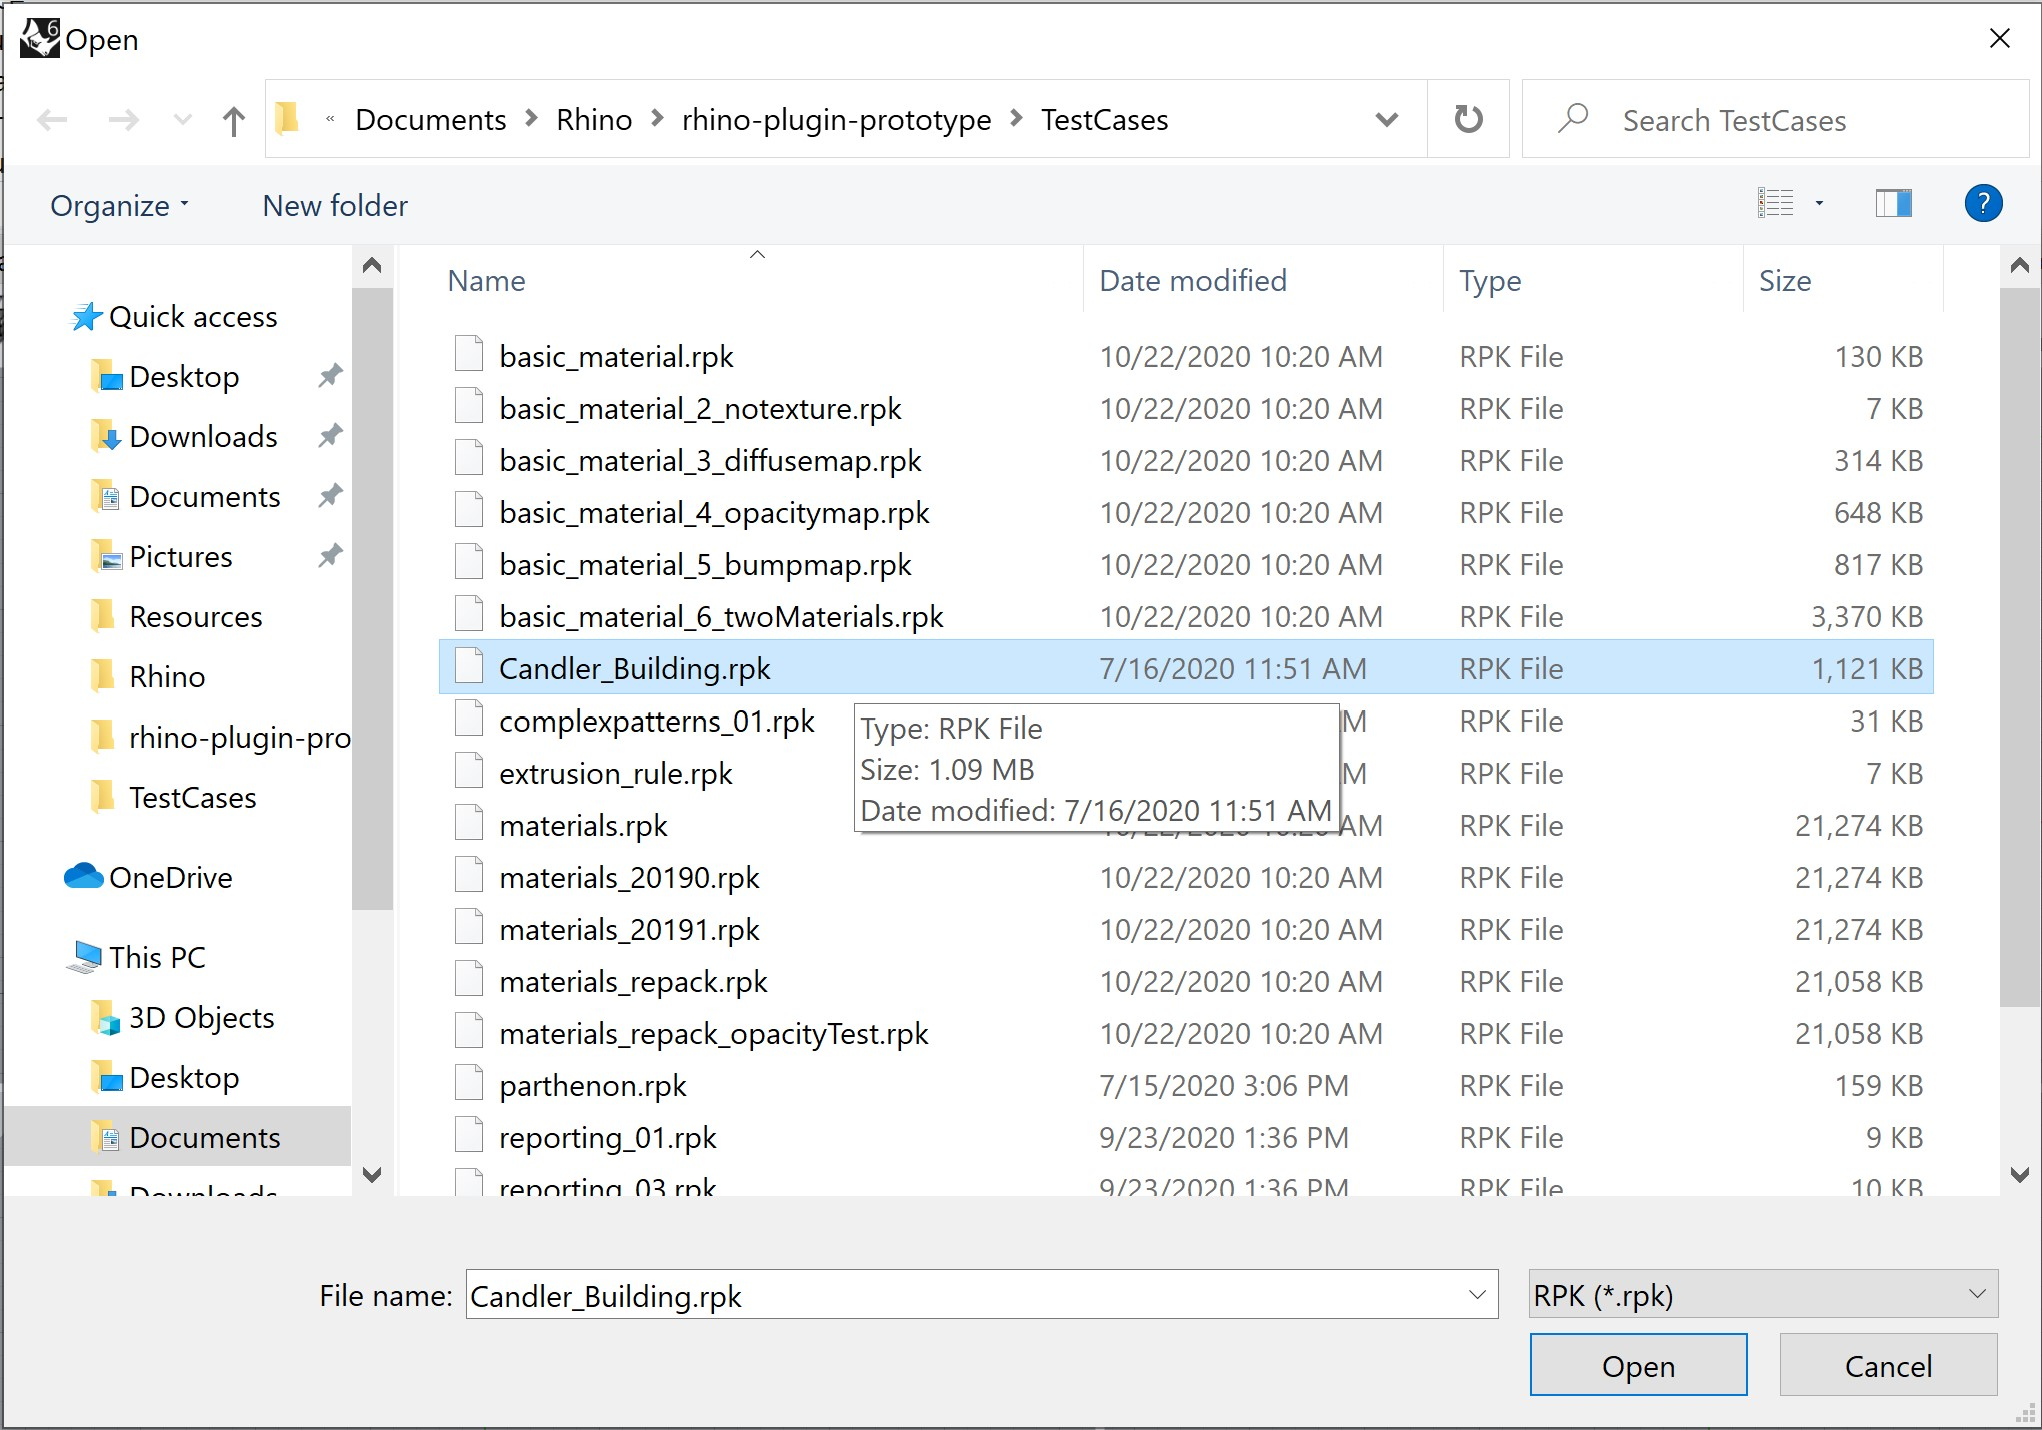
\includegraphics[width=10cm]{res/man_rhino_rpk_browser}
        \captionof{figure}{Choose a rule package.}
    \end{minipage}
    \newpage
    \item Select one or more starting shapes then press enter.\\
    \begin{minipage}{\linewidth}
        \centering
        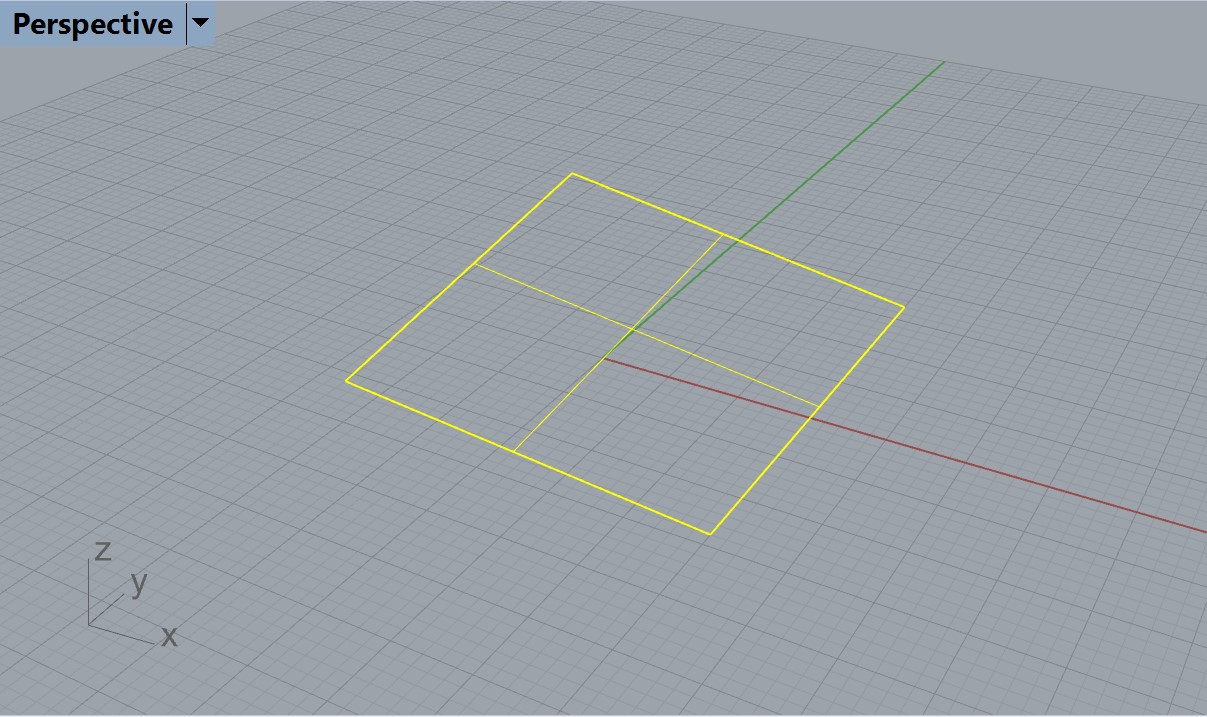
\includegraphics[width=9cm]{res/man_rhino_pick_shape}
        \captionof{figure}{Select one or more starting shapes.}
    \end{minipage}
    \item The resulting geometry will be generated and appear in the Rhino viewport.\\
    \begin{minipage}{\linewidth}
        \centering
        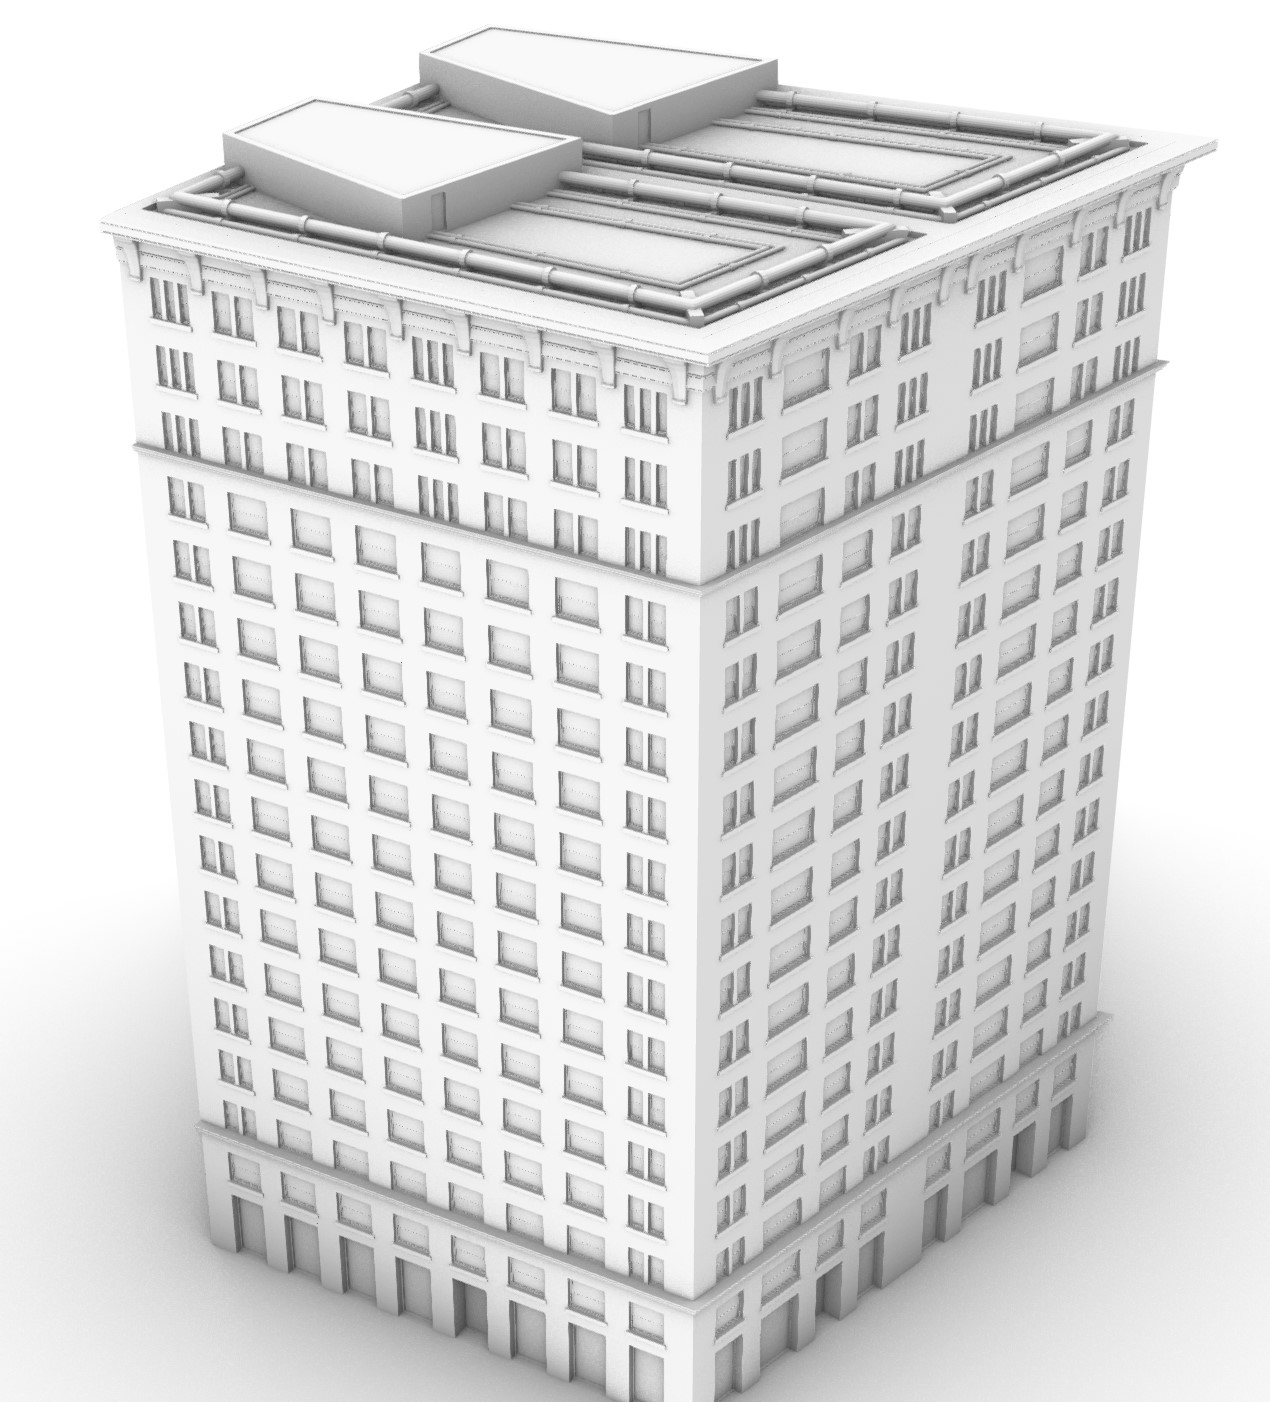
\includegraphics[width=9cm]{res/man_rhino_cmd_result}
        \captionof{figure}{Example of resulting geometry.}
    \end{minipage}
\end{enumerate}

